\documentclass[12pt]{article}
\usepackage[margin=1in]{geometry}
\usepackage{graphicx}
\usepackage{setspace}
\usepackage{url}

\title{Tecellate: A Distributed Environment for Ad Hoc Wireless Network Simulations}
\author{
        Steve Johnson (srj15@case.edu)\\
        Case Western Reserve University\\
        \and Tim Henderson (tah35@case.edu)\\
        Case Western Reserve University
}
\date{\today}

\begin{document}
\doublespacing
\maketitle

% \begin{multicols}{2}

\begin{abstract}
    Tecellate is a simulation in which autonomous agents can move in a grid and communicate using
    semi-realistic radio signals. The simulation itself can be distributed over multiple machines to
    allow for very large simulations. The system allows researchers to test various wireless network
    protocols and algorithms under arbitrarily harsh conditions.
    
    The usefulness of the simulation was tested using an approximated IP stack. Our initial results
    show that the simulation produces useful information, though more work is required to improve
    its accuracy and suitability for research.
\end{abstract}

\section{Introduction}

Computer network modeling and simulation has become an important tool in the arsenal of any computer
networks researcher. It has only become more important as increasingly research into mobile
and autonomous devices matures. Large scale simulations of thousands to hundreds of thousands of
devices become increasingly crucial to validate techniques without having to spend thousands of
dollars on costly equipment. To support such simulations we present Tecellate, a horizontally
scalable distributed network simulator.

Tecellate simulates the physical layer of the network. All \textbf{agents} (actors in the
simulation) have a ``radio'' to send and receive byte strings. To approximate the real world, these
byte strings may be probabilistically corrupted as a function of distance and interference. To
provide reliable communication between arbitrary agents, users must implement the link, IP, and
transport layers. As a resource to users wishing to model the traditional TCP/IP stack the authors
provide a partial implementation up to the IP layer.\footnote{
  We hope to expand this implementation to include the TCP and UDP transport layers as well.
}

In the physical world, devices move around with purpose and transmit with purpose. We assert that
the same should be true in a simulation. However, modeling the purpose of actual people is not
possible. Therefore, the simulation gives the agents an alternative purpose: to stay alive. Each
agent has to ``eat'' in order to survive. Each turn, each agent may eat a unit of food if its
current location contains food. If it runs out of food, it dies. The goal of the agents is to stay
alive as long as possible. Thus, it must find sources of food within the simulation. This game-like
element provides the agents with goals and a purpose for communication.

As wireless networks become more widespread, the number of participants in a given network will
grow. Simulations that are not scalable may become too slow to simulate important test cases. For
this reason, Tecellate is designed to scale horizontally across many machines.

By modeling the communication at the physical layer and adding game-like elements to our simulation,
we hope to provide an interesting test bed for networking and AI algorithms. The game-like element
in our simulation will help ensure the agents move around purposefully in the simulation grid. The
physical layer simulation ensures that the communication problems which must be overcome for
reliable communication are similar to real world problems. The inherent scalability of the system
should allow simulation of arbitrarily large scenarios. While, we do not think our simulation
approach would be the final word in networks simulation, it should provide a useful platform for
experimentation.

\section{Literature Survey}

There are a few existing simulations of wireless ad hoc networks that operate above the link layer.
One of these is ns2, which has been around for several years \cite{ns2}. ns2 simulates multiple
kinds of networks and protocols, and it has been popular among researchers. However, it is difficult
to scale above a few hundred nodes \cite{swans}. It has only been documented to scale to a few
thousand nodes.

GloMoSim is a newer simulator \cite{glomosim}. It serves a similar purpose to ns2 and can simulate
both wired and wireless networks, but it is more scalable in that it can run its event loop in
parallel \cite{swans}. It can scale to tens of thousands of nodes.

SWANS is a simulator created purely for ad hoc wireless network research in response to the
inadequacy of ns2 and GloMoSim for ad hoc wireless network research \cite{swans}. It has a different
configuration/modeling style from other solutions which allows it to accurately simulate millions of
nodes on 2004 hardware.

A specialized wireless ad hoc network simulator is $madhoc$, a system that attempts to accurately
model wireless network characteristics in metropolitan settings \cite{madhoc}. The authors argue
that other simulators' node movement algorithms do not accurately model real world environments, and
consequently spend a great deal of effort modeling the characteristics of metropolitan environments.

These simulators differ from Tecellate in that they simulate a higher level of the network and
provide no inherent goal for communicating agents. They also simulate radio signal propagation much
more accurately, which affects the computation requirements drastically. They have sophisticated
physics-based models of signal strength which must be updated and accounted for when sending and
receiving transmissions, while we propose to use simpler probabilistic methods at the bit level.


\section{Simulation Rules} \label{rules}

The simulation runs in discrete steps (\textbf{turns}). The conceptual ``length'' of a turn is
designed to simulate the time to send $k$ bytes, where $k$ is a configurable constant. Each turn, an agent may do any combination of the following: listen, broadcast, move, or die.

\subsection{Movement}

The simulation world consists of a $w$*$h$ grid of signed integers. If a cell's value $c$ is
non-negative, it is the terrain height. Otherwise, the cell is impassable. An agent can move at most
one cell up, down, left, or right per turn. However, after moving into a square, it must wait $c$
turns before it may make another move.

An agent's move may succeed or fail. If an agent tries to move into an impassible cell, it will
fail. It will also fail if it tries to move into a cell that was occupied by another agent at the
end of the last turn, \textbf{or} a cell that another agent attemps to move into in the same turn.
These cases are shown in figure \ref{mvt}.

\begin{figure*}[h!]
    \begin{center}
        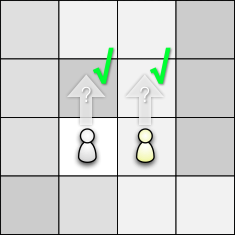
\includegraphics[width=1in]{figures/mvt1.png}
        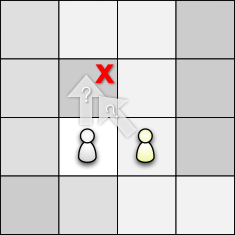
\includegraphics[width=1in]{figures/mvt2.png}
        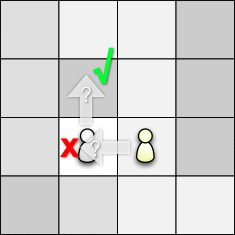
\includegraphics[width=1in]{figures/mvt3.png}
    \end{center}
    \caption{Three main cases for movement.}
    \label{mvt}
\end{figure*}

It may seem more intuitive for both moves in case 3 to succeed, i.e. a move $Z\rightarrow Y$ should
succeed if agent $A$ moves $X\rightarrow Y$. However, allowing this case would introduce large
dependency graphs that would span a large geographical area. This kind of dependency graph would
greatly reduce the effectiveness of our horizontal scaling scheme based on geographical partitioning
described later in this paper.

\subsection{Messages}

The broadcast messages agents can send are a simpilification of radio communication. There are $N$
frequencies an agent can broadcast on or listen too. An agent may broadcast a message of 1024 bytes
on a single frequency. The agent may also listen for messages on $M$ frequencies each turn where $M
\leq N$.

Like radio communication, the messages broadcast decay over distance. When an agent listens to a
frequency, the agent always recieves data. However, if no one is broadcasting on that frequency, the
agent will recieve random data. Since the message decays over distance, even if an agent hears it
some parts of the message may be corrupted. The farther away a listener is from a sender, the more
corruption is in the message.

Finally, if more than one message can be heard from the same position, the messages will be combined
probabilistically.

% Finally, if messages cross each other the following algorithm will be used to resolve the
% conflict. First, for each message the message will be corrupted based on its distance to its source,
% just as in the single broadcaster senario. Then, for each bit in each message their will be a
% probability K that the bit will be heard. The probablity will also be based on the distance to the
% source of the message. All of the bits that are heard are XORed together creating a composite
% message. If not bit are heard for a particular bit location a random value is chosen for that bit.

\subsection{Perception}

Agents may or may not be informed of their global position in the world. They also have some way of
``seeing'' nearby agents.

\subsection{Food}

Agents must search the grid to find food. If their coordinator calculates that their food counter is
below zero, they disappear from the grid.

\section{Usefulness of the Simulation}

The simulation provides a close enough approximation of the real world to allow testing of
high-level coordination algorithms to be tested using a very simple API.

The rules for movement (1 delayed turn per cell height difference) and perception provide an
opportunity to experiment with pathfinding algorithms in an environment where little information
outside a limited area is available, similar to the conditions of the DARPA autonomous vehicle
events.

The rules for communication force agents to communicate with distant agents by passing messages
through nearby agents, creating ad-hoc wireless networks. Our messaging system is meant to model the
difficulties of real world radio communication. This will make our simulation a useful tool for
simulating adhoc wireless networks allowing protocol research to be conducted without hardware.


\section{System Architecture}

The system can operate in one of two modes. In local mode, the simulation runs in one process with a
scenario defined in code. The remote mode is described below.

\subsection{Distributed Architecture}

\begin{figure*}
    \begin{center}
        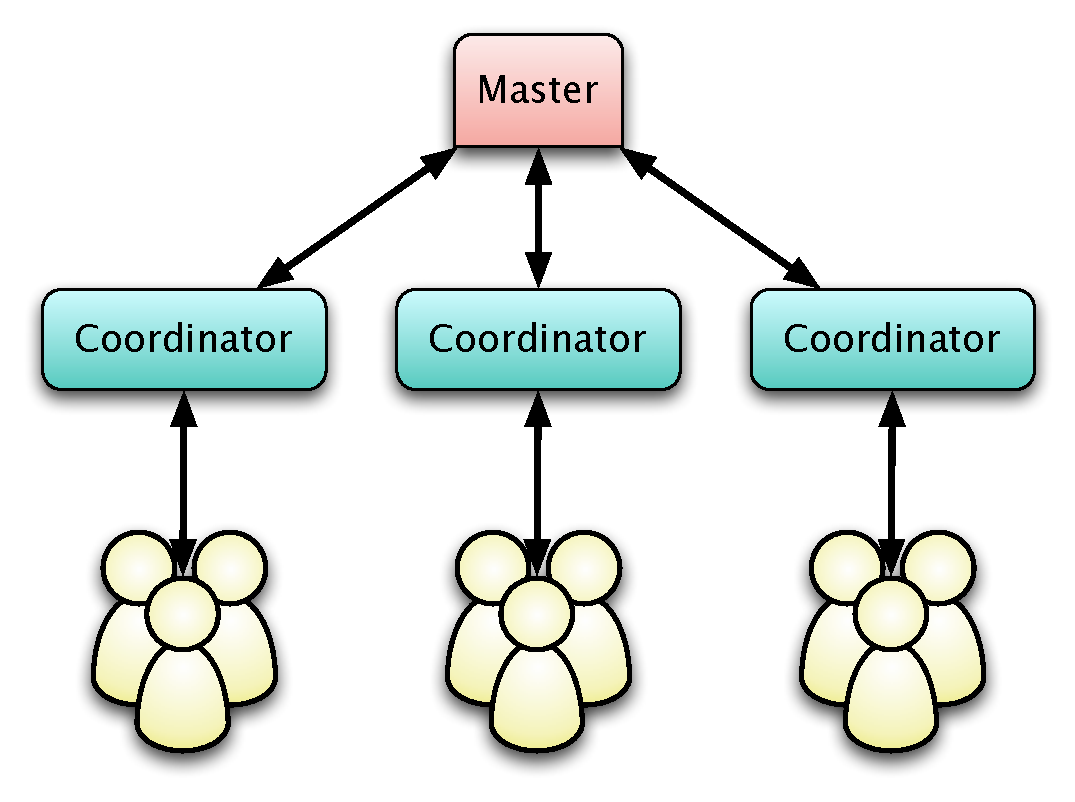
\includegraphics[width=3in]{figures/arch0.pdf}
    \end{center}
    \caption{Basic architecture of the system.}
    \label{arch}
\end{figure*}

In order to support simulations on the scale of millions of agents, Tecellate can be run in a
distributed mode on many machines. Individual components communicate via TCP. The architecture of
this distributed version is shown in figure \ref{arch}.

\begin{figure*}
    \begin{center}
        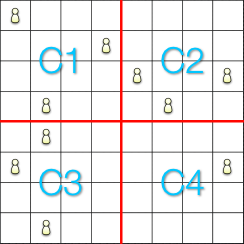
\includegraphics[width=3in]{figures/arch1.png}
    \end{center}
    \caption{Grid-based method for distributing work across coordinators}
    \label{geoarch}
\end{figure*}

Agents are run in individual processes. In order to interact with the simulation, they connect to a
\textbf{coordinator}. Coordinators are responsible for evaluating discrete grid sections each turn
and communicating their results to each other when relevant. The organization of a square grid
section is shown in figure \ref{geoarch}.

The simulation starts with all agent and coordinator processes waiting and listening at individual
addresses. A master process reads a configuration file with their addresses and initial states,
sends information about how to connect to each other, waits for the connections to finish, and
instructs the coordinators to begin the simulation. It then exits and the other processes log
simulation data to configurable log files.

Each coordinator is responsible for a rectangular section of the grid. These sections are assigned
at the start of the simulation and do not change. Coordinators are connected with neighbor
coordinators that share adjacent grid sections. When an agent moves from one grid section to
another, the agent connects to the coordinator responsible for the new section.

\subsection{Coordinator Implementation Details}

There are two main types of threads associated with each coordinator. One kind of thread (A-thread)
requests agent data from neighbors, and then applies the simulation rules to the agents's previous
states based on their requested actions and the states of the agents at the neighbor coordinators.
There is only one of these threads. The other kind of thread (B-thread) serves requests for agent
information from neighbors, and there is one of these for each neighbor ($|N|$).

The A-thread and the B-threads communicate using two semaphores, \textbf{turnAvailable} and
\textbf{requestsServed}. The A-thread signals \textbf{turnAvailable} $|N|$ times when a turn has
been processed, and the B-threads each wait on it before serving a new request. When a B-thread has
served a request, it signals \textbf{requestsServed}. The A-thread waits on \textbf{requestsServed}
before it begins processing a new turn to avoid overwriting data that B-threads are still serving.
The system starts with \textbf{turnAvailable} unlocked for the B-threads.

This system allows processing and RPC serving to run in parallel, with processing running one step
ahead of RPC serving.

Processing a turn (in the A-thread) involves exchanging messages with each agent to get its moves
for the next turn. This may happen over TCP or in-memory communication channels depending on the
mode of operation.

\subsection{Issues and Possible Improvements}

The biggest issue with the current implementation is that distributed communication via TCP is
orders of magnitude slower than communication in memory. While this limiation is not surprising, it
is probably possible to improve communication speed by switching to a UDP-based protocol.

The application is highly multithreaded even within individual components. A modest run will have 40
or more threads. These are not OS-level threads but rather lightweight runtime-level threads.
Despite their lightweight nature, a large proportion are waiting for input most of the time, for
example to serve an RPC request. Our educated guess is that 60\% of threads are in this state at any
given moment. These threads may be wasting more CPU cycles than necessary when they are scheduled.

Performance improves when the language runtime is instructed to split the threads across multiple
CPU cores, but when this is done, a major memory leak manifests which makes the system unusable.
This memory leak may be caused by the language runtime, but we are still investigating the issue.

If agents cluster in one geographic area, one coordinator may have a significantly higher burden
than the others. This problem could be solved by allowing the master process to dynamically
reallocate the space assigned to each coordinator. This dynamic reassignment is very similar to the
problem of assigning many application instances to many servers, but in addition to simply trying to
distribute CPU and memory load evenly, we are also trying keep traffic between coordinators to a
minimum. It would take another paper to describe an effective algorithm to accomplish this goal, and
probably a simulator-simulator to test it.

\subsection{Use of the Go Programming Language}

This project would have been much more difficult without the use of the new programming language Go.
First released by Google in November 2009 \cite{go_new}, Go is a systems programming language with
C-like syntax, garbage collection, concurrency primitives, basic object orientation, and lightweight
threads. This code example shows the unique features of Go that made Tecellate easier to write:

\begin{tscode}
\begin{verbatim}
package main

import "fmt"

func main() {
    // Declare two "channels", one for strings (for communication) and 
    //      another one to serve as a mutex to allow the main thread 
    //      to wait until the other threads finish before exiting
    comm := make(chan string)
    can_exit := make(chan bool)
    
    // Start a thread that sends a message down the communication channel
    go func(send_chan chan string) {
        send_chan <- "hello"
    }(comm)
    
    // Start another thread that receives the message and tells the
    //      main thread to exit
    go func(recv_chan chan string, done chan bool) {
        val := <- recv_chan
        fmt.Printf("Received from sender: '%v'\n", val)
        done <- true
    }(comm, can_exit)
    
    // Wait for the receive thread to signal exit
    <- can_exit
}
\end{verbatim}
\end{tscode}

This code snippet demonstrates \textbf{goroutines} and \textbf{channels}. A goroutine is a
lightweight thread that is scheduled by the runtime. A channel is a thread-safe way to pass data
from one point to another. The code snippet demonstrates the use of one channel to pass a string to
display, and another channel to act as a mutex to stop the main thread from exiting before all work
is complete.

The standard library provides a way to attach a channel to a TCP connection. This library is what
allows us to easily switch between local and distributed modes of operation.


\section{Validation}

iaweofiaw efoaw iefj



\section{Conclusion}

This project has three layers. At the top layer, we want to refine a system that distributes work among several servers. At the middle layer, we want to implement a simulation. At the bottom layer, we want to use it as a testbed for ad-hoc wireless networks. For these reasons, we think it is a compelling course project.


\nocite{*}
\bibliographystyle{acm}
\bibliography{bibliography}

\end{document}
